\documentclass[times, utf8, diplomski]{fer}
\usepackage{booktabs}
\usepackage{color}
\usepackage{listings}
\usepackage{pdfpages}
\usepackage{subcaption}
\usepackage{float}

\graphicspath{ {./resources/images/} }

\lstset{ %
language=C++,                % choose the language of the code
basicstyle=\footnotesize,       % the size of the fonts that are used for the code
numbers=left,                   % where to put the line-numbers
numberstyle=\footnotesize,      % the size of the fonts that are used for the line-numbers
stepnumber=1,                   % the step between two line-numbers. If it is 1 each line will be numbered
numbersep=5pt,                  % how far the line-numbers are from the code
backgroundcolor=\color{white},  % choose the background color. You must add \usepackage{color}
showspaces=false,               % show spaces adding particular underscores
showstringspaces=false,         % underline spaces within strings
showtabs=false,                 % show tabs within strings adding particular underscores
frame=single,           % adds a frame around the code
tabsize=2,          % sets default tabsize to 2 spaces
captionpos=b,           % sets the caption-position to bottom
breaklines=true,        % sets automatic line breaking
breakatwhitespace=false,    % sets if automatic breaks should only happen at whitespace
escapeinside={\%*}{*)}          % if you want to add a comment within your code
}

\begin{document}

% TODO: Navedite broj rada.
\thesisnumber{2926}

% TODO: Navedite naslov rada.
\title{3D interaktivna vizualizacija simulacije vibracija}

\author{Nikola Vugdelija}

\maketitle

% Ispis stranice s napomenom o umetanju izvornika rada.
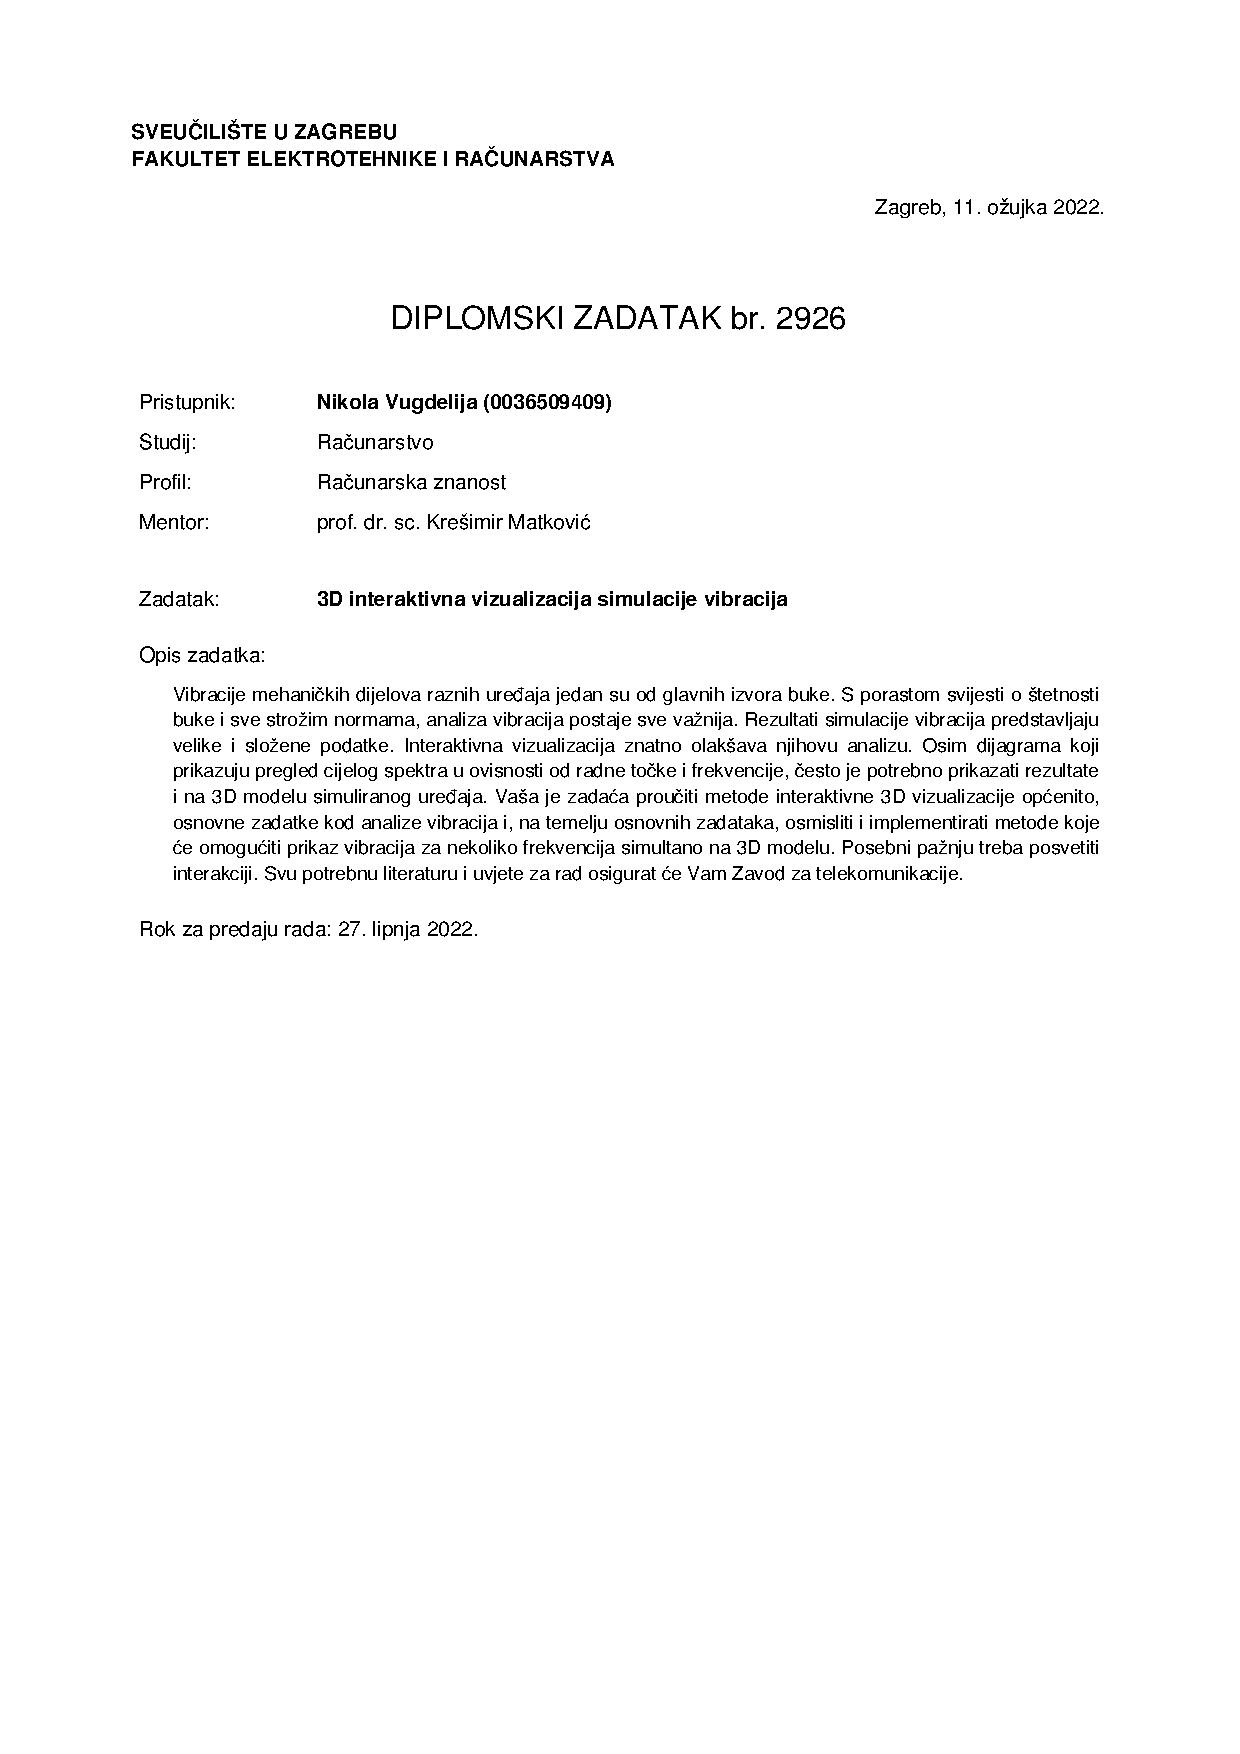
\includepdf[pages=-]{resources/docs/task.pdf}


% Dodavanje zahvale ili prazne stranice. Ako ne želite dodati zahvalu, naredbu ostavite radi prazne stranice.
\zahvala{Zahvala će biti ovdje kad je formuliram u glavi.}

\tableofcontents

\listoffigures

\chapter{Uvod}
Buka i vibriranje motora su jedni od ključnih faktora koji utječu na osjećaj udobnosti putnika u osobnom automobilu. No, iako se može reći kako je osjećaj udobnosti subjektivne prirode, propisi koji kontroliraju dozvoljene razine buke motora vozila pri određenim brzinama su objektivni i egzaktni. Zbog navedenih razloga je inženjerima iznimno važno da je vibriranje motora prilikom rada na što nižoj razini, a najjednostavniji način na koji to mogu provjeriti u fazi projektiranja motora je pomoću NVH \engl{Noise, Vibration, Harshness} simulacija. NVH simulacije inženjerima omogućuju precizan uvid u razinu vibriranja pojedinih dijelova motora, a probleme koji mogu uzrokovati vibraciju mogu rješavati prilikom projektiranja.\\

No, računanje simulacije je samo dio problema. Računske simulacije ove vrste, nerijetko proizvode podatke koje se ne može jednostavno vizualizirati i analizirati \citep{matkovic2021getting}. Kako bi stručnjaci mogli navedene podatke koristiti na što efikasniji način, potrebno ih je intuitivno i razumljivo prikazati. Iako su podaci prikazani u obliku tablica i grafova korisni, vizualizacijom istih podataka na 3D modelu motora se postiže jasniji, intuitivniji i potpuniji prikaz rada motora.\\

Ovaj rad opisuje izradu alata za vizualizaciju podataka dobivenih iz NVH simulacije pomoću 3D modela motora i 2D grafova. Fokus predstavljenog alata je na vizualizaciji vibracija motora prilikom rada na višestrukom broju frekvencija, kako bi se razine vibracije različitih taktova motora jednostavnije uspoređivale.

\chapter{Pregled područja}
Iako često zanemarena, vizualizacija podataka je iznimno važno područje analize podataka. Pošto isti skup podataka može prenijeti potpuno drugačije informacije ovisno o načinu prikaza, od velike je važnosti odabrati optimalne vizualizacijske tehnike za konkretni skup podataka. Ali kako je naglašeno u \citep{Unwin2020Why}, kod vizualizacije ne postoji jedna, "optimalna" grafika koja vrijedi za svaki skup podataka, nego je često potrebno pronaći grupu vizualizacijskih tehnika koje se međusobno upotpunjuju i prikazuju cjelovitu sliku. Stoga je tijekom osmišljavanja alata za vizualizaciju izrazito važno utvrditi za koju svrhu se taj alat koristi, te koje informacije je potrebno njime vizualizirati iz danog skupa podataka. Odgovori na navedena pitanja postaju kompleksniji za odgonetnuti s porastom kompleksnosti skupa podataka koji alat vizualizira. Zbog toga je pomoć stručnjaka u domeni itekako korisna.\\

Kao što je već spomenuto, glavna svrha alata razvijenog u sklopu ovog rada je vizualizacija NVH podataka na modelu motora. Prilikom izrade ovog rada je korišten isti skup podataka koji je korišten kod \citep{matkovic2021getting}. Spomenuti podaci su izračunati NVH simulacijom pomoću alata AVL EXCITE™\citep{avlEXCITE}. Motor je zadan kao skup ćelija, a za svaku ćeliju su poznate koordinate okolnih točaka u 3D prostoru, te kojom snagom ćelija vibrira pri različitim frekvencijama rada.\\

Kako je spomenuto u \citep{matkovic2021getting}, stručnjake pri analizi NVH podataka ponajprije zanimaju tri stavke:

\begin{itemize}
\item Usporedba podataka na različitim frekvencijama rada
	\begin{itemize}
	\item Kako se vibracije mijenjaju sa promjenom frekvencije rada motora?
	\end{itemize} 
\item Lokalizacija značajki
	\begin{itemize}
	\item Koje ćelije motora pri zadanoj frekvenciji vibriraju iznosom koji pripada zadanom rasponu?
	\end{itemize} 
\item Lokalna pretraga
	\begin{itemize}
	\item Kojom snagom vibriraju odabrane ćelije?\\
	\end{itemize} 
\end{itemize}

Alat razvijen u \citep{matkovic2021getting} dobro adresira navedene značajke. Koristeći paralelne koordinate, omogućen je detaljan pregled usporedbe podataka na različitim frekvencijama. Adresiranje druge i treće značajke je olakšano omogućavanjem korištenja višestrukih, međusobno povezanih prozora sa 3D prikazom motora. Lokalna pretraga je ostvarena uz pomoć "kista", kojeg korisnik može koristiti za biranje raspona iznosa vibracija za određene frekvencije, a svi prozori automatski ažuriraju prikaz modela motora označujući ćelije koje pripadaju zadanim rasponima. Konačno, u \citep{matkovic2021getting} je lokalna pretraga omogućena bojanjem modela motora bazirano na vrijednostima vibracija pojedinačnih ćelija pri radu na zadanoj frekvenciji. Detaljniji uvid u snagu vibriranja pojedine ćelije modela je omogućen odabirom interesne ćelije, nakon čega se istakne 2D graf vibracija  zadane ćelije.\\

No, iako je referirani rad cjelokupno odlično pokrio sve tri značajke, u području usporedbe podataka na različitim frekvencijama rada još ima prostora za napredak. Naime, trenutna usporedba podataka na različitim frekvencijama je moguća samo pomoću 2D grafova, koji iako korisni, imaju problema sa čitljivošću i jasnoćom. Alat koji je razvijen u sklopu ovog rada implementira niz vizualizacijskih tehnika koje potencijalno povećavaju intuitivnost usporedbe vibracija motora na različitim frekvencijama u odnosu na izvedbu kod \citep{matkovic2021getting}.

\chapter{Analiza zadatka i zahtjeva}
Pošto dizajniranje alata za vizualizaciju nije jednostavan zadatak, potrebno je poduzeti određene predprodukcijske korake kako bi se osigurala zadovoljavajuća implementacija glavnog zadatka. Navedeni je zadatak potrebno dodatno analizirati, čime bi se uočili zahtjevi potrebni za njegovo uspješno odrađivanje. Identificirane zahtjeve je također potrebno analizirati, kako bi se utvrdila njihova povezanost sa glavnim zadatkom, te osiguralo njihovo uspješno i cjelovito zadovoljavanje. 

\section{Identificirani zadaci}
Ključni zadatak alata razvijenog u sklopu ovog rada je prikazivanje razlika i sličnosti između različith frekvencija rada ćelija motora na intuitivan i razumljiv način. Kao što je već navedeno u prethodnom poglavlju, alat iz \citep{matkovic2021getting} ima problema sa čitljivošću i jasnoćom usporedbe utjecaja više frekvencija na vibraciju motora. Spomenuta usporedba je jedino moguća korištenjem grafova kod kojih svaka linija predstavlja funkciju vibracije jedne ćelije (x-os predstavlja sve frekvencije za koje postoje podaci, a y-os predstavlja snagu vibracije). Takav način rada stvara nezanemarive poteškoće sa korištenjem alata: teže je usporediti frekvencije koje nisu susjedne na grafu, čitljivost grafa je uvelike smanjena kada je odabrano više ćelija i otežano je uočiti gdje se točno na modelu motora nalaze razlike u radu motora.

\section{Identificirani zahtjevi} \label{requests-section}
Kako bi se usporedbu učinilo intuitivnijom i jasnijom, očiti korak je omogućiti iscrtavanje rezultata usporedbe na 3D modelu motora. Naime, iako se u \citep{matkovic2021getting} ćelije bojaju na temelju jačine vibracija pri radu na zadanoj frekvenciji, nije moguće iscrtati utjecaj više frekvencija na modelu motora. Takvim iscrtavanjem bi se uveliko olakšalo uočavanje promjena na dijelovima motora. Naravno, kod više odabranih frekvencija, postavlja se pitanje: kako iz niza podataka o snagama vibracije ćelija pri odabranim frekvencijama odabrati jedan konačni iznos koji će pomoću zadanog raspona i gradijenta odrediti konačnu boju ćelije kojoj pripada. Alat razvijen u sklopu ovog rada korisniku nudi nekoliko funkcija koje može odabrati, a koje primaju niz iznosa vibracija te vraćaju jednu vrijednost vibracije, koja predstavlja "sažetak" navedenog niza. Za tu svrhu su u sklopu alata implementirane metode:

\begin{itemize}
\item MIN - najmanji iznos vibracije
\item MAX - najveći iznos 
\item AVERAGE - prosjek vibracija
\item MEDIAN - medijan vibracije
\item SPREAD - razlika između najvećeg i najmanjeg iznosa vibracije\\
\end{itemize}

Korisnik zatim može odabrati funkciju koja najbolje odgovara njegovim potrebama. Na primjer, ako korisnik treba saznati maksimalno opterećenje za svaku ćeliju pri odabiru različitih frekvencija za to mu može koristiti funkcija MAX, a ako ga zanima kolike će vibriranje ćelija varirati tijekom rada na višestrukim frekvencijama može koristiti funkciju SPREAD itd.\\

No, kada navedene funkcije iz niza vrijednosti izračunaju konačnu vrijednost, taj iznos treba prebaciti u interval [0, 1] kako bi se omogućilo uzorkovanje gradijenta. Za ostvarivanje prijelaza u taj interval potrebno je znati koji broj označava najmanju vrijednost intervala, odnosno 0, a koji broj označava najveću vrijednost intervala, odnosno 1. U alatu su ponuđena tri načina računanja navedenog raspona:
\begin{itemize}
\item GLOBAL - donju i gornju granicu raspona čine najmanji i najveći iznos snage vibracije kojom neka ćelija može vibrirati tijekom rada na bilo kojoj od mogućih frekvencija
\item LOCAL - donju i gornju granicu raspona čine najmanji i najveći iznos snage vibracije kojom neka ćelija može vibrirati tijekom rada na bilo kojoj od odabranih frekvencija
\item USER DEFINED - korisnik sam definira donju i gornju granicu raspona\\
\end{itemize}

Alat korisniku omogućuje da sam definira boje gradijenta na temelju kojeg će se modelu odrediti boje ćelija.\\

U sklopu alata je implementiran još jedan način "bojanja" modela motora koji je baziran na unaprijed određenim ograničenjima vibracija. Navedena ograničenja dijele raspon vibracija na 3 zone: bezopasnu, rizičnu i opasnu. Rasponi su definirani za određene frekvencije (ne nužno za sve) u posebnoj datoteci. Ovaj način bojanja je odvojen od normalnog načina rada, objašnjenog u prijašnjem odlomku. Boje ćelija u načinu rada s ograničenjima se određuju na sljedeći način:
\begin{itemize}
\item Zelena - ako se snaga vibracije trenutne ćelije tijekom rada na svim odabranim frekvencijama nalazi u bezopasnoj zoni
\item Gradijent žute - ako se snaga vibracije trenutne ćelije tijekom rada na barem jednoj odabranoj frekvenciji nalazi u rizičnoj zoni, a nijedna u opasnoj zoni
\item Gradijent crvene - ako se snaga vibracije trenutne ćelije tijekom rada na barem jednoj odabranoj frekvenciji nalazi u opasnoj zoni\\
\end{itemize}

Navedeni gradijenti se uzorkuju pomoću omjera broja frekvencija prilikom kojih snaga vibracije ćelije spada u zonu gradijenta i ukupnog broj odabranih frekvencija. Navedena boja i gradijenti su početno postavljeni na spomenute vrijednosti, a korisnik ih može mijenjati kako njemu odgovara.\\

Kako bi se adresirao problem sa uspoređivanjem nesusjednih frekvencija, na grafu se iscrtavaju samo podaci za odabrane frekvencije. Konačno, kako bi se poboljšala čitljivost grafa u sklopu alata su implementirana dva načina iscrtavanja podataka: stupčasti i linijski, te tri načina uspoređivanja:
\begin{itemize}
\item DEFAULT - svi grafovi su prikazani unutar jednog prikaza
\item SUBPLOTS - svaki graf je prikazan unutar zasebnog prikaza
\item RELATIVE - kao DEFAULT, ali je dodatno moguće odabrati jednu ćeliju s obzirom na koju će se prikazati grafovi svih ostalih ćelija\\
\end{itemize}

Navedeno rješenje predstavlja poboljšanje na području čitljivosti zbog više razloga. Grafovi svih ćelija više nisu prikazani odjednom, već su samo prikazani grafovi odabranih ćelija. Moguće je prikazati svaki graf na zasebnom prikazu, čime je pojednostavljeno uspoređivanje u slučaju više odabranih ćelija. Sa relativnim uspoređivanjem, korisnik može lakše usporediti odabranu ćeliju sa ostalim ćelijama. Konačno, pošto su omogućena dva načina iscrtavanja podataka, korisnik može odabrati način koji najbolje odgovara njegovim potrebama i preferencijama, te nije prisiljen koristiti linije za iscrtavanje grafova.

\chapter{Dizajn vizualizacije}

Zahtjevi navedeni u prijašnjem poglavlju daju naslutiti kako će sučelje alata biti kompleksno, pošto korisniku trebaju biti na raspolaganju brojne opcije. Kako bi se svi navedeni zahtjevi zadovoljili, a upotrebljivost alata se ne bi smanjila, potrebno je alat organizirati u smislene prozore, koje će korisnik moći premiještati, povećavati i smanjivati kako mu najbolje odgovara. Na slici \ref{fig:gen-screen} se može vidjeti kako je alat zapravo organiziran u sedam prozora. Navedeni prozori su detaljno opisani u nastavku.\\

\begin{figure}[H]
\centering
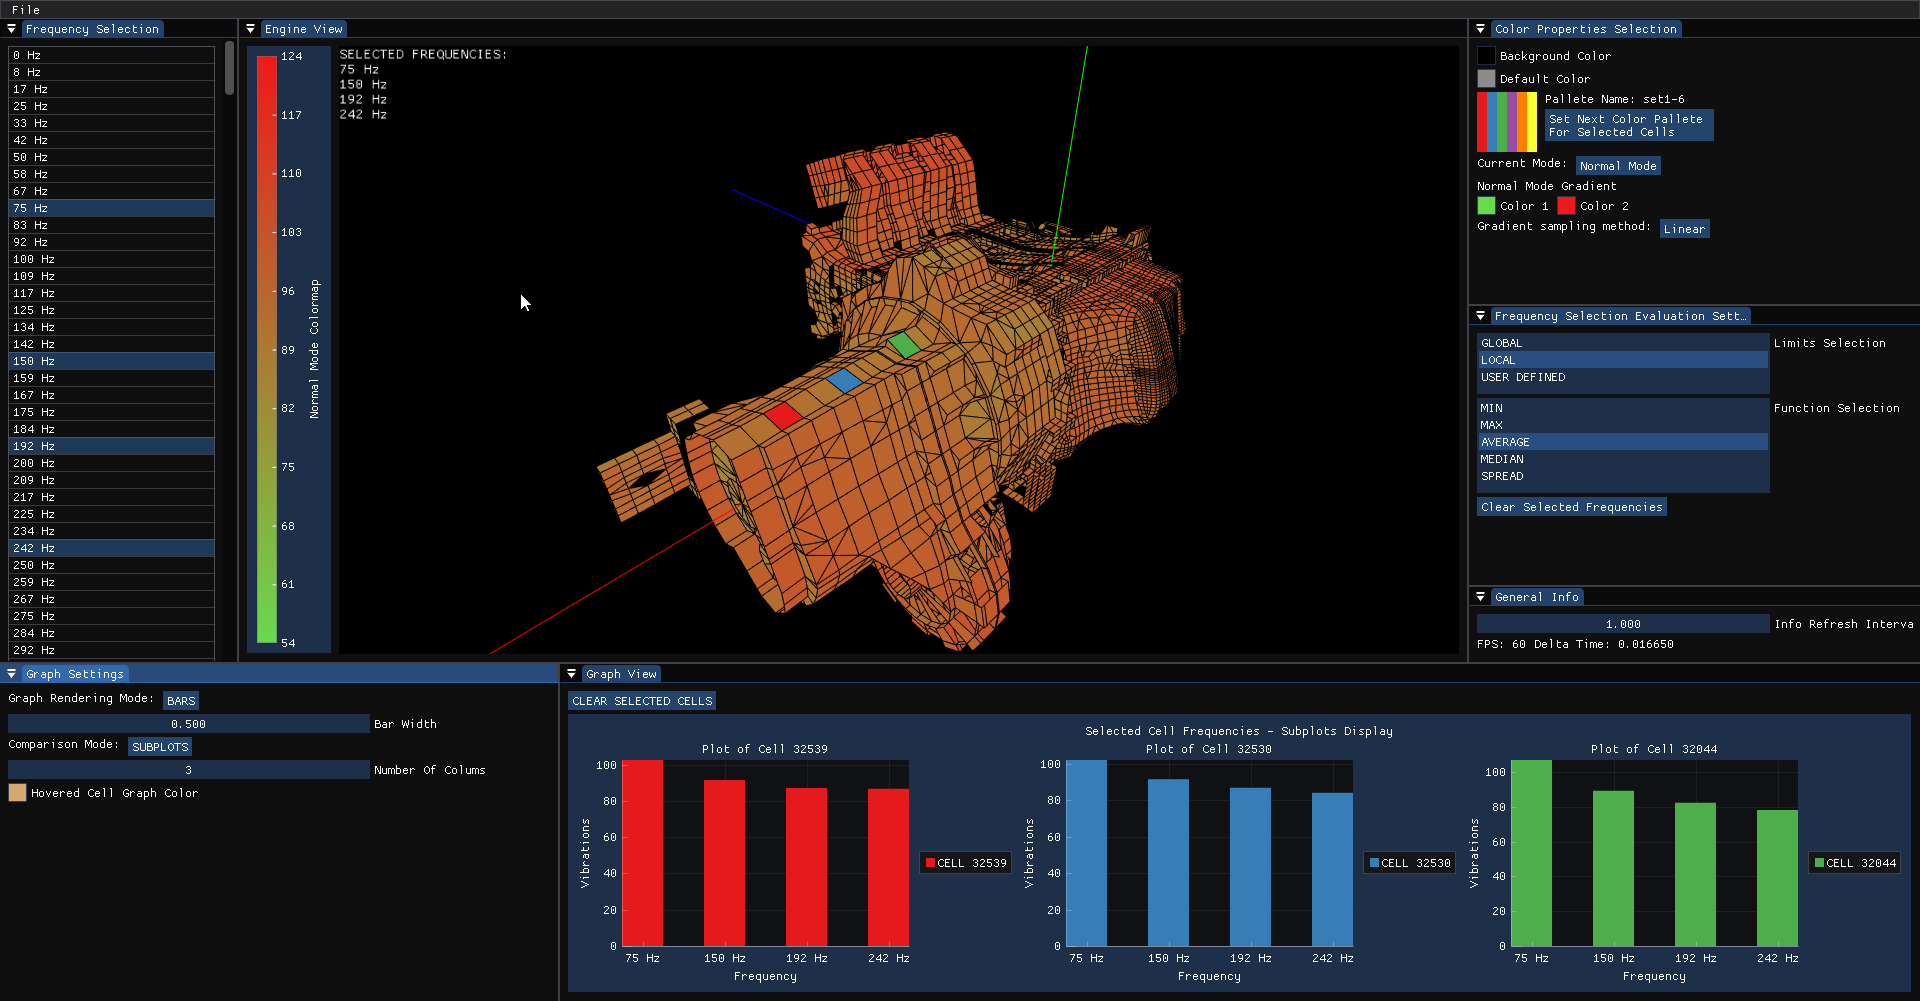
\includegraphics[width=\linewidth]{general_screenshot.png}
\caption{Snimka zaslona alata}
\label{fig:gen-screen}
\end{figure}

\section{Prikaz motora} \label{engine-view-section}
Zadaća prikaza motora je jasno vizualizirati podatke o vibracijama ćelija, pritom uzimajući u obzir brojne postavke vizualizacije poput: načina rada, odabranih frekvencija, načina računanja konačnih podataka ćelije, zadanih raspona podataka, gradijenata koje se koristi za vizualizaciju i načina uzorkovanja tih gradijenata. Korisnik ovu komponentu također može koristiti i za označavanje interesnih ćelija.\\
\begin{figure}[H]
\centering
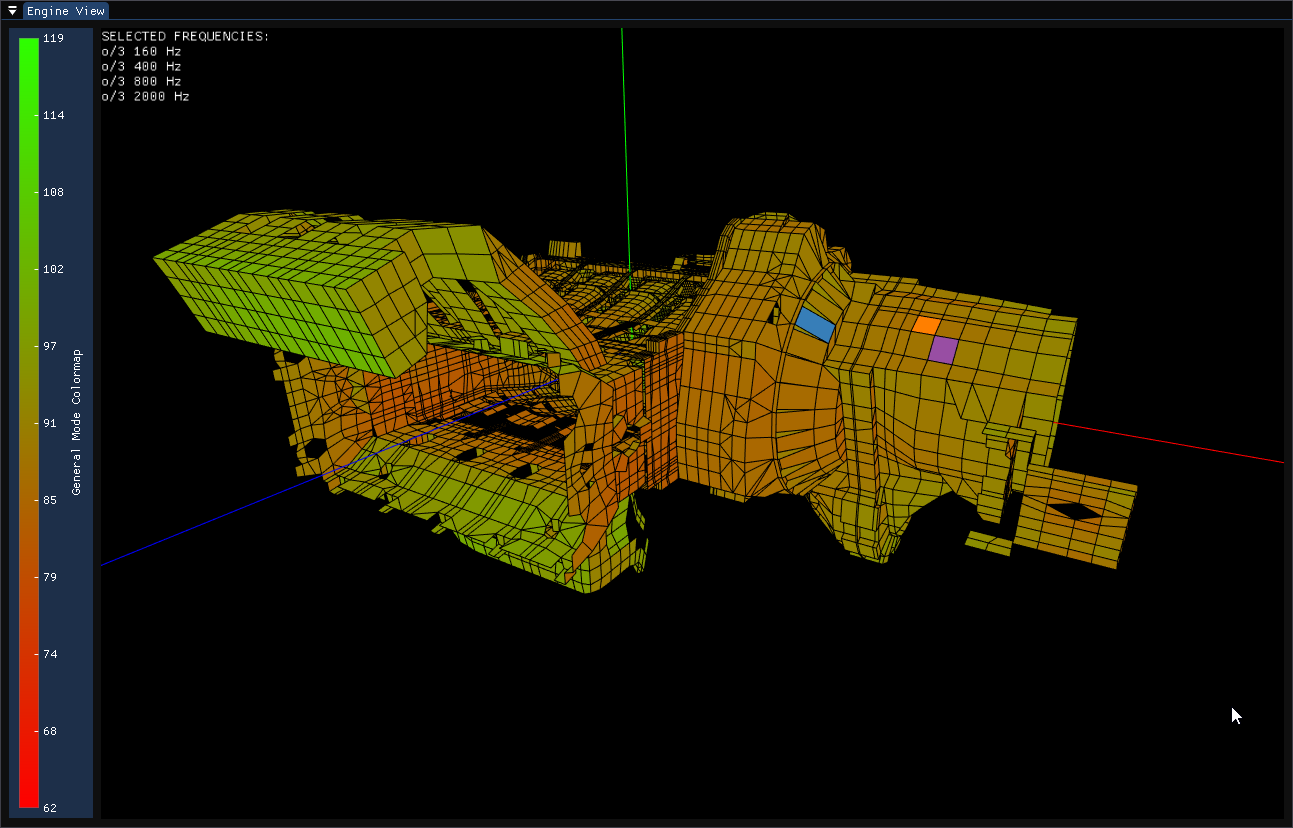
\includegraphics[width=0.85\linewidth]{engine_view_normal_mode.png}
\caption{Prikaz motora tijekom normalnog načina rada}
\label{fig:normal-mode-engine-view}
\end{figure}
\begin{figure}[h]
\centering
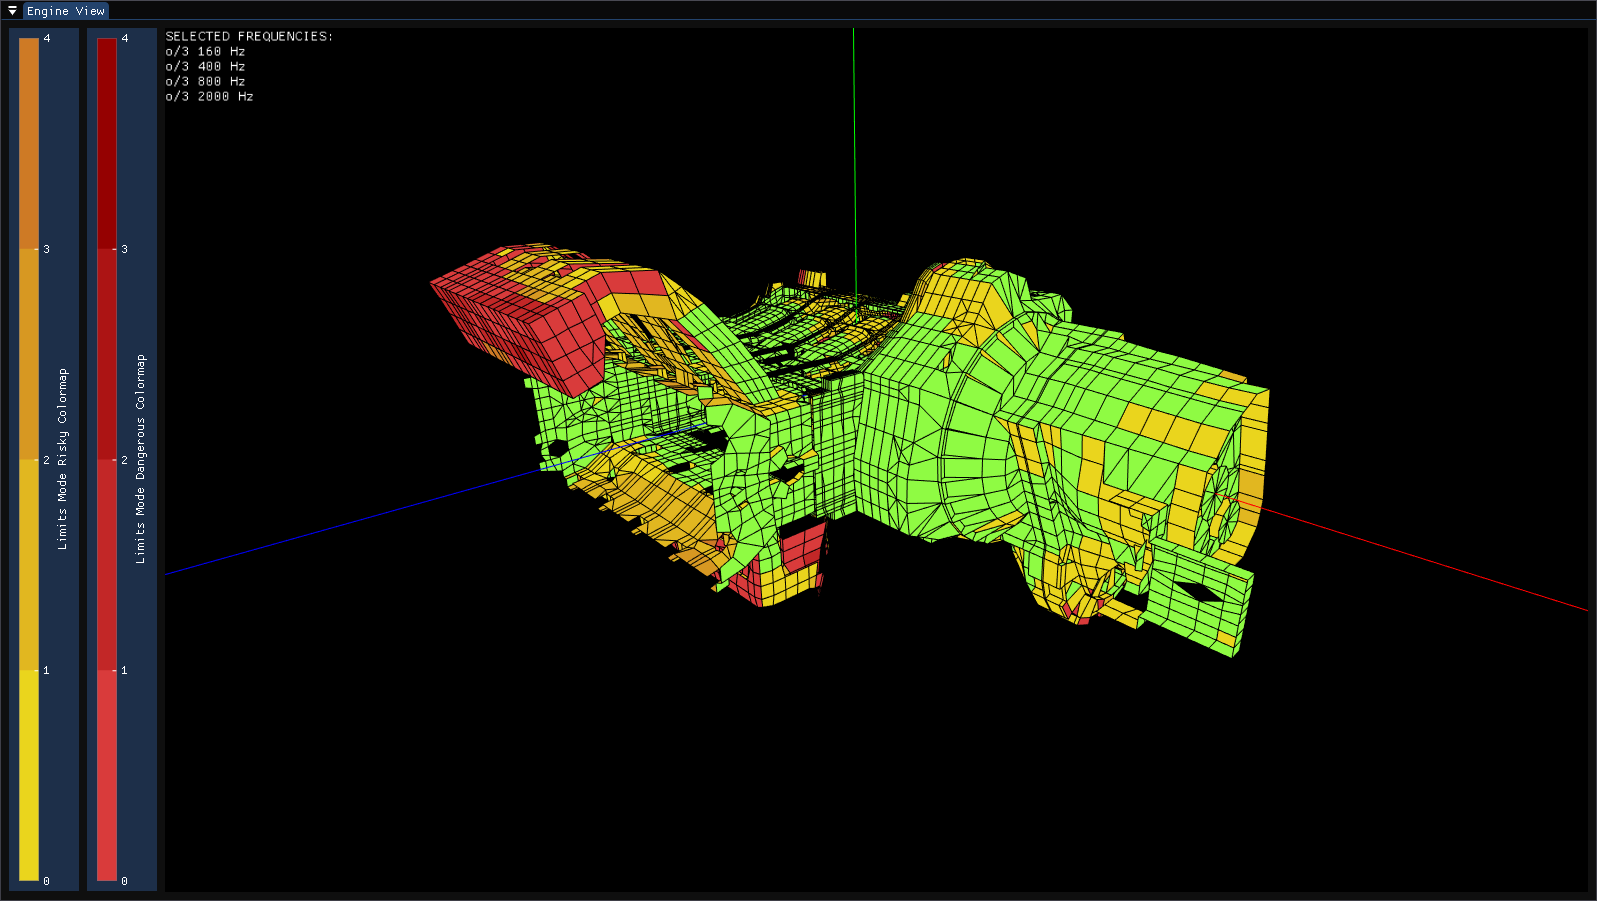
\includegraphics[width=0.85\linewidth]{engine_view_limits.png}
\caption{Prikaz motora tijekom načina rada sa preddefiniranim ograničenjima}
\label{fig:limits-mode-engine-view}
\end{figure}

Na slikama \ref{fig:normal-mode-engine-view} i \ref{fig:limits-mode-engine-view} se može vidjeti primjer ovog prikaza tijekom dva moguća načina rada. Uz prikaz obojanog modela ova komponenta alata je zadužena i za prikaz legende gradijenta i nabrajanje odabranih frekvencija, kako bi snimak prikaza prenosio sve relevantne informacije potrebne za razumijevanje rezultata vizualizacije. Osi koordinatnog sustava su nacrtane uz model motora kako bi korisnik dobio osjećaj za 3D prostor u kojem se model nalazi. Označavanje ćelija se odrađuje pozicioniranjem pokazivača miša iznad interesne ćelije te klikom na lijevu tipku miša. Kada korisnik pokazivačem miša prijeđe preko ćelije bez klikanja, boja ćelije postaje inverz prijašnje boje, kako bi se korisniku dala povratna informacija o ćeliji koja će biti odabrana odluči li se korisnik kliknuti lijevu tipku miša. Opisana ćelija će se u nastavku rada nazivati "lebdeća" ćelija. Jednom kada korisnik klikne na ćeliju, ćelija se označava jednom od boja iz trenutne palete (detaljno objašnjeno u poglavlju \ref{color-settings-section}) te je korisniku prikazan detaljan uvid u podatke označene ćelije putem prikaza grafa (vidi poglavlje \ref{graph-view-section}). Ponovnim klikom na već odabranu ćeliju, ćelija se briše iz liste odabranih ćelija.\\

Kao što je vidljivo iz slika \ref{fig:normal-mode-engine-view} i \ref{fig:limits-mode-engine-view}, razlike u dva načina rada se ne manifestiraju samo u vizualizaciji motora, već i u sučelju ovog prikaza. Naime, kako je objašnjeno u poglavlju \ref{requests-section}, u normalnom načinu rada alatu je potreban jedan kontinuirani gradijent, a u načinu rada sa preddefiniranim ograničenjima su potrebna dva diskretna gradijenta.
\begin{figure} [H]
     \centering
     \begin{subfigure}[h]{0.16\textwidth}
         \centering
         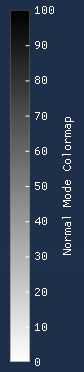
\includegraphics[width=\textwidth]{linear_colormap.png}
         \caption{Linearno}
         \label{fig:linear_legend}
     \end{subfigure}
     \hfill
     \begin{subfigure}[h]{0.16\textwidth}
         \centering
         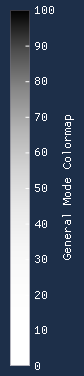
\includegraphics[width=\textwidth]{cubic_colormap.png}
         \caption{Kubno v1}
         \label{fig:cubic_legend}
     \end{subfigure}
     \hfill
     \begin{subfigure}[h]{0.16\textwidth}
         \centering
         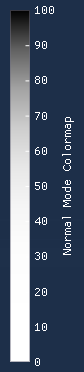
\includegraphics[width=\textwidth]{quartic_colormap.png}
         \caption{Kvartičko v1}
         \label{fig:quartic_legend}
     \end{subfigure}
     \hfill
     \begin{subfigure}[h]{0.16\textwidth}
         \centering
         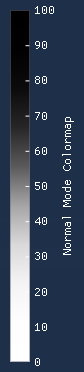
\includegraphics[width=\textwidth]{cubic_symmetrical_colormap.png}
         \caption{Kubno v2}
         \label{fig:cubic_symmetrical_legend}
     \end{subfigure}
     \hfill
     \begin{subfigure}[h]{0.16\textwidth}
         \centering
         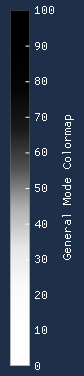
\includegraphics[width=\textwidth]{quartic_symmetrical_colormap.png}
         \caption{Kvartičko v2}
         \label{fig:quartic_symmetrical_legend}
     \end{subfigure}
        \caption{Drugačije postavke uzorkovanja gradijenta\\}
        \label{fig:colormap-legends}
\end{figure}

Osim što je navedene gradijente moguće mijenjati pomoću dvije kontrolne boje, moguće ih je mijenjati i promjenom funkcije uzorkovanja gradijenta, a utjecaj različitih funkcija uzorkovanja na kontinuirane gradijente se može vidjeti na slici \ref{fig:colormap-legends}. Različite funkcije uzorkovanja su direktno preuzete sa \citep{easing}.

\section{Prikaz grafa} \label{graph-view-section}

Komponenta prikaza grafa služi za iscrtavanje jednog ili više prikaza grafova odabranih ćelija, ali i "lebdeće" ćelije. Prilikom iscrtavanja spomenutih grafova uzimaju se u obzir brojne postavke i načini crtanja. Boje grafova odabranih ćelija odgovaraju bojama koje te ćelije imaju unutar prikaza motora (vidi poglavlje \ref{engine-view-section}), a boja grafa "lebdeće" ćelije je zadana unutar postavki grafa (vidi poglavlje \ref{graph-settings-section}). Kao što je navedeno u poglavlju \ref{requests-section}, alat implementira tri načina usporedbe i dva načina iscrtavanja grafova, a izgled ove komponente uz sve moguće kombinacije postavki grafa su prikazane na slikama u dodatku \ref{appendix:graph-display-examples}. Na navedenim slikama se može vidjeti kako ovu komponentu čini jedan ili više prikaza grafova i gumb za brisanje liste odabranih ćelija.\\

Sa slika u dodatku \ref{appendix:graph-display-examples} je također vidljivo kako su rasponi osi prikaza grafova postavljeni tako da obuhvaćaju podatke koji se u njima nalaze, te nisu fiksno određeni. Implementacija ovakvog načina određivanja raspona je odabrana zbog smanjene preglednosti razlika u "tokovima" grafova kada su postavljeni fiskni rasponi, pošto pri fiksnim rasponima grafovi zauzimaju puno manji dio prikaza, a ostatak prikaza je potrošen na prazan prostor. Spomenuta primjedba je posebno uočljiva na slikama \ref{appendix:subplots_graph_display_bars} i \ref{appendix:subplots_graph_display_lines} gdje se vidi kako, zbog različitih raspona, grafovi koji su iscrtani pomoću stupaca bolje pokazuju razliku u iznosima podataka, ali grafovi iscrtani pomoću linija bolje pokazuju razlike u "tokovima" grafova. Konkretno, na slici \ref{appendix:subplots_graph_display_bars} se na prvi pogled čini kako se zelena ćelija (ćelija 10982) i žuta ćelija (ćelija 11182) ponašaju slično, no uvidom u graf na slici \ref{appendix:subplots_graph_display_lines} se otkriva kako to nije istina. Ali ako se korisniku ovakav način određivanja raspona ne sviđa, u alatu je moguće otvoriti postavke bilo koje osi prikaza grafa pozicioniranjem pokazivača miša iznad željene osi te klikom na desnu tipku miša. Kao što se vidi na slici \ref{fig:graph-axis-settings}, unutar spomenutih postavki je moguće uređivati brojna svojstva osi poput raspona, načina interpoliranja između granica raspona, smjera osi i mnoge druge postavke.

\begin{figure} [H]
	\centering
    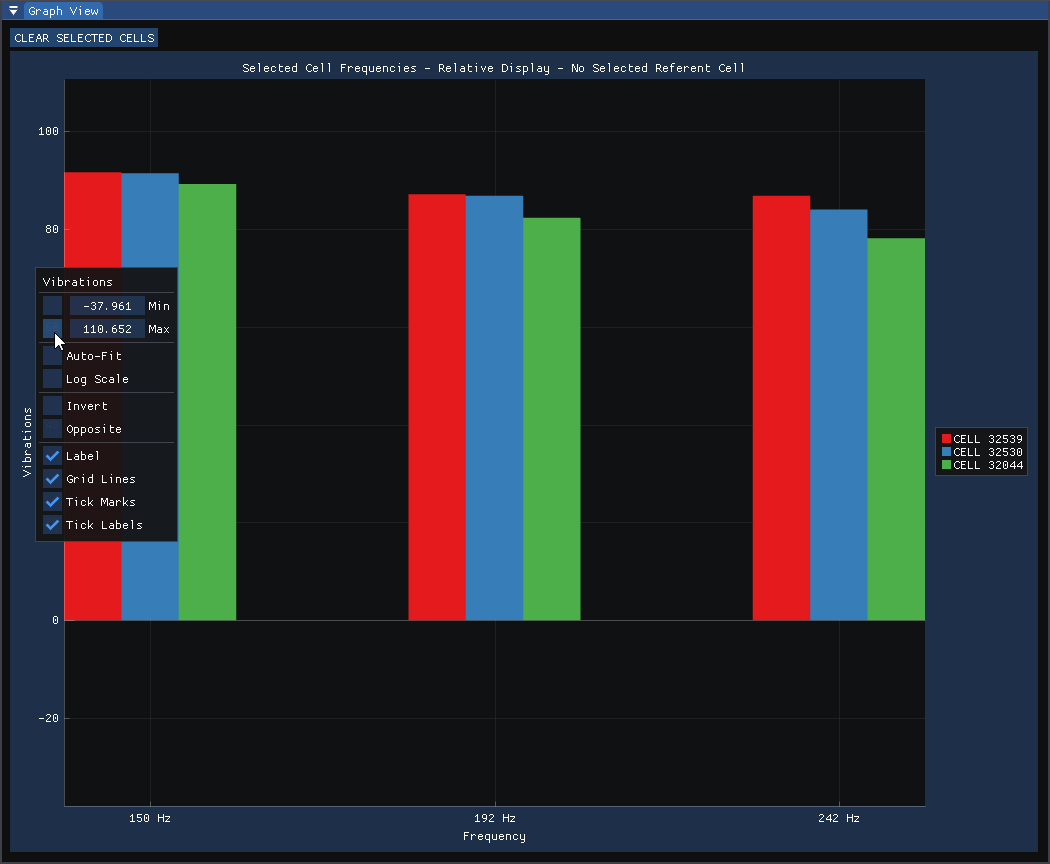
\includegraphics[width=\textwidth]{graph_view_axis_settings.png}
    \caption{Postavke osi prikaza grafa}
    \label{fig:graph-axis-settings}
\end{figure}

\section{Postavke boja} \label{color-settings-section}
Kao što samo ime ove komponente kaže, glavna svrha joj je čuvanje postavki koje bi mijenjale boje i gradijente unutar prikaza motora. Na slici \ref{fig:color-settings-2-modes} mogu se vidjeti razlike u komponenti između dva moguća načina rada. U oba načina rada moguće je promijeniti pozadinsku boju prikaza motora, početnu boju motora (boju koju motor ima kad nijedna frekvencija nije odabrana), paletu za odabrane ćelije i trenutni način rada. No dva prikaza postavki boja se ipak djelomično razlikuju, pošto je za normalni način rada potrebno definirati samo jedan gradijent, a za način rada sa preddefiniranim ograničenjima je potrebno definirati jednu boju (za sigurnu zonu) i dva gradijenta (za rizičnu i opasnu zonu).

\begin{figure} [H]
     \centering
     \begin{subfigure}[h]{0.49\textwidth}
         \centering
         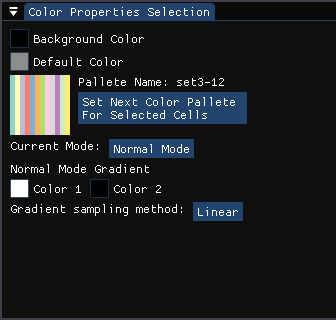
\includegraphics[width=\textwidth]{color_settings_normal_mode.png}
         \caption{Normalni način rada}
         \label{fig:color-settings-normal-mode}
     \end{subfigure}
     \hfill
     \begin{subfigure}[h]{0.49\textwidth}
         \centering
         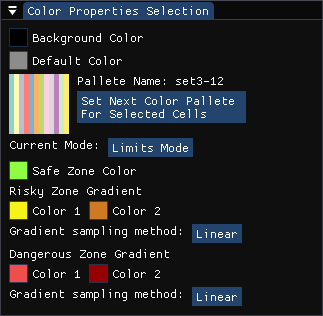
\includegraphics[width=\textwidth]{color_settings_limits_mode.png}
         \caption{Način rada sa preddefiniranim ograničenjima}
         \label{fig:color-settings-limits-mode}
     \end{subfigure}
     \caption{Postavke boja tijekom dva moguća načina rada\\}
     \label{fig:color-settings-2-modes}
\end{figure}

Što se tiče mijenjanja postavki, korisnik može mijenjati boje klikom na obojani kvadrat čime se otvara prozor za mijenjanje boja prikazan na slici \ref{fig:color-picker}. U otvorenom prozoru boju se može mijenjati pomoću interaktivnog GUI sučelja ili unosom RGB ili HSV vrijednosti boje, a također je moguće i unošenje boja u heksadekadskom formatu.\\

\begin{figure} [H]
	\centering
    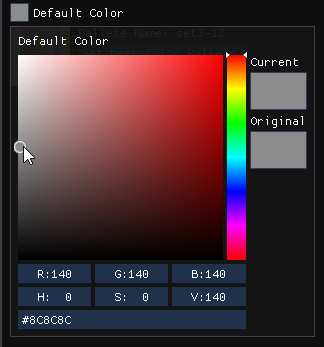
\includegraphics[width=0.5\textwidth]{color_settings_color_picker.png}
    \caption{Prozor za odabir boje\\}
    \label{fig:color-picker}
\end{figure}

Palete boja za odabrane ćelije su učitane izravno iz datoteke \textit{default\_pallete.txt} koja se mora nalaziti u istom direktoriju kao i izvršna datoteka alata. Početne palete su preuzete sa \citep{colorbrewer} i unesene u navedenu datoteku u sljedećem formatu:

\begin{lstlisting}
p ime_palete
rgb_vrijednosti_boje1_u_rasponu_0_255
rgb_vrijednosti_boje2_u_rasponu_0_255
rgb_vrijednosti_boje3_u_rasponu_0_255
rgb_vrijednosti_boje4_u_rasponu_0_255
\end{lstlisting}
\ \\

Na slici \ref{fig:color-settings-2-modes} se može vidjeti kako je za svaku paletu u kvadratiću prikazan spektar boja, desno od kojeg je navedeno ime palete, a ispod imena se nalazi gumb za prelazak na sljedeću paletu. Kako palete sadrže ograničen broj boja, u alatu je implementiran način brisanja ćelija kada je broj odabranih ćelija veći od broja boja u paleti. Postoje dva slučaja kod kojih se to dogodi: pri dodavanju nove ćelije kada su već sve boje palete "zauzete" i pri mijenjanju trenutne palete na paletu čiji je broj boja manji od broja trenutno odabranih ćelija. U prvom slučaju alat briše zadnju odabranu ćeliju i dodaje novoodabranu ćeliju, a u drugom slučaju alat briše onoliko zadnjih odabranih ćelija kolika je razlika između broja odabranih ćelija i broja boja nove palete.\\

Ispod sučelja za mijenjanje palete se nalazi gumb za mijenjanje načina rada. Na gumbu piše ime trenutnog načina rada, a klikom na gumb alat prelazi u sljedeći način rada. Kako su moguća samo dva načina rada, gumb će alternirati između normalnog načina rada i načina rada sa preddefiniranim ograničenjima.\\

Konačno, sučelje za odabir gradijenta se sastoji od dva standardna kvadrata za mijenjanje boja pomoću kojih se mijenja početna i krajnja kontrolna boja gradijenta. Ispod navedenih kvadrata se nalazi gumb za mijenjanje metode uzorkovanja gradijenta. Implementirane metode uzorkovanja i njihov utjecaj na gradijent su objašnjene i prikazane u poglavlju \ref{graph-view-section}.

\section{Postavke grafa} \label{graph-settings-section}

Postavke grafa se dijele na tri dijela koji su jasno naznačeni na slici \ref{fig:graph-settings-segmented}. Dio u kojem se mijenja boja grafa lebdeće ćelije se ne mijenja s obzirom na različite načine crtanja ili uspoređivanja jer se taj graf uvijek iscrtava. Kao što je već napomenuto u poglavlju \ref{requests-section}, alat implementira dva načina iscrtavanja grafa: linijski i stupčasti, a razlika u postavkama između ta dva načina je što stupčastom grafu korisnik može odrediti širinu stupca, kao što se može vidjeti na slici \ref{fig:graph-settings-segmented}, dok na linijskom grafu korisnik ne može mijenjati ništa. Način iscrtavanja se mijenja klikom na gumb na kojem piše ime trenutno aktivnog načina iscrtavanja.

\begin{figure} [H]
	\centering
    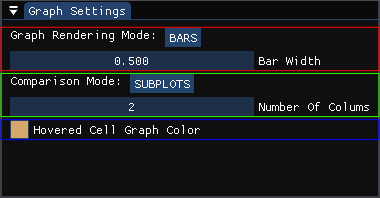
\includegraphics[width=0.7\textwidth]{graph_settings_subplots_segmented.png}
    \caption{Postavke grafa rastavljene na dijelove: postavke načina iscrtavanja (crveno), postavke načina usporedbe (zeleno) i postavke boje grafa "lebdeće ćelije" (plavo)}
    \label{fig:graph-settings-segmented}
\end{figure}

Ali za razliku od postavki načina iscrtavanja, razlike između postavki načina uspoređivanja su puno uočljivije. Tijekom normalnog načina usporedbe, korisnik nema nikakvih dodatnih postavki osim gumba za mijenjanje načina usporedbe koji je prisutan tijekom svih načina uspoređivanja i funkcionira na identičan način kao i gumb za mijenjanje načina iscrtavanja. Tijekom načina usporedbe sa višestrukim prikazima, korisnik može odabrati u koliko će se stupaca prikazi organizirati. Konačno, kada je aktivan relativni način usporedbe, korisnik može odabrati jednu od već odabranih ćelija s obzirom na koju će se prikazati grafovi ostalih ćelija. Gumb ćelije koju korisnik odabere, ali i gumb ćelije iznad koje korisnik postavi pokazivač miša poprima boju odgovarajuće ćelije iz prikaza motora. Navedeni dodatak je implementiran kako bi korisnik imao bolju ideju o tome koja ćelija je trenutno odabrana i/ili koja će ćelija biti odabrana za relativno iscrtavanje.

\begin{figure} [H]
     \centering
     \begin{subfigure}[h]{0.48\textwidth}
         \centering
         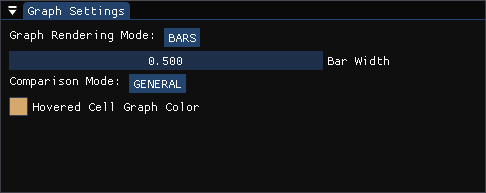
\includegraphics[width=\textwidth]{graph_settings_default.png}
         \caption{Normalni način usporedbe}
         \label{fig:graph-settings-normal-mode}
     \end{subfigure}
     \hfill
     \begin{subfigure}[h]{0.48\textwidth}
         \centering
         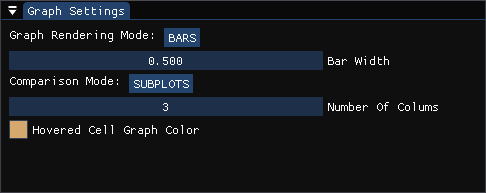
\includegraphics[width=\textwidth]{graph_settings_subplots.png}
         \caption{Način usporedbe sa višestrukim prikazima}
         \label{fig:graph-settings-limits-mode}
     \end{subfigure}
     \hfill
     \begin{subfigure}[h]{0.48\textwidth}
         \centering
         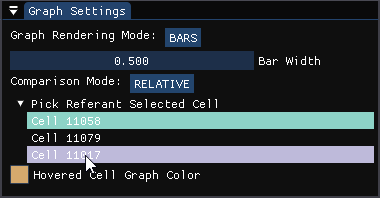
\includegraphics[width=\textwidth]{graph_settings_relative.png}
         \caption{Relativni način usporedbe}
         \label{fig:graph-settings-limits-mode}
     \end{subfigure}
     \caption{Postavke grafa tijekom tri različita načina usporedbe}
     \label{fig:graph-settings-3-modes}
\end{figure}

\section{Odabir frekvencija} \label{frequency-selection-section}

Ova komponenta služi isključivo za odabir frekvencija (kao što i samo ime govori), a postavljena je u odvojenu komponentu od postavki evaluacije odabranih frekvencija (opisanih u poglavlju \ref{frequency-settings-section}) radi poboljšanja lakoće korištenja alata. Izgled komponente se može vidjeti na slici \ref{fig:frequency-selection-view}. U normalnom načinu rada komponenta prikazuje sve frekvencije za koje su učitani podaci o vibriranju ćelija, dok su u načinu rada sa preddefiniranim ograničenjima prikazane samo frekvencije za koje je definirano ograničenje u datoteci sa ograničenjima. 

\begin{figure} [H]
	\centering
    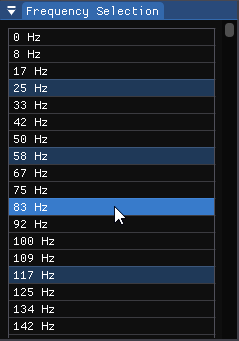
\includegraphics[width=0.45\textwidth]{frequency_selection_view.png}
    \caption{Prozor za odabir frekvencija}
    \label{fig:frequency-selection-view}
\end{figure}

\section{Postavke evaluacije odabranih frekvencija} \label{frequency-settings-section}

Kao što je već opisano u poglavlju \ref{requests-section}, korisnik u normalnom načinu rada može dodatno prilagoditi prikaz utjecaja odabranih frekvencija na vibraciju motora odabirom različitih metoda pomoću kojih se iz niza podataka o vibraciji ćelije dobije jedan konkretan podatak, ali i odabirom raspona pomoću kojeg se izračunati podatak pretvori u podatak iz raspona [0, 1] kako bi se olakšalo uzorkovanje gradijenta. Navedene prilagodbe nisu moguće prilikom načina rada sa preddefiniranim ograničenjima, pošto je algoritam već "strogo" zadan i nema dijelova algoritma koje korisnik može mijenjati, ali spomenute parametre normalnog načina rada, korisnik može mijenjati unutar komponente postavki odabranih frekvencija koja je prikazana na slici \ref{fig:frq-sel-eval-settings}.

\begin{figure} [H]
	\centering
    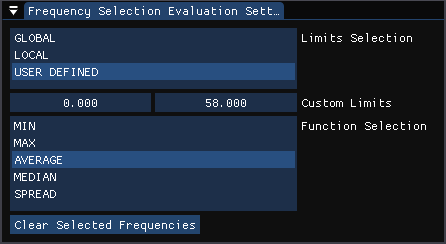
\includegraphics[width=0.8\textwidth]{frq_sel_eval_settings.png}
    \caption{Prozor postavki evaluacije odabranih frekvencija sa svim mogućim parametrima}
    \label{fig:frq-sel-eval-settings}
\end{figure}

Prozor postavki evaluacije odabranih frekvencija nije vidljiv sve dok korisnik ne odabere jednu od ponuđenih frekvencija unutar komponente iz poglavlja \ref{frequency-selection-section}. Kada se odabere barem jedna frekvencija, prozor postavki se prikazuje sa parametrima koji su vidljivi ovisno o broju odabranih frekvencija i načinu rada u kojem korisnik koristi alat.\\

Oba načina rada u postavkama imaju gumb za brisanje liste trenutno odabranih frekvencija. Način rada sa preddefiniranim ograničenjima osim tog gumba u postavkama neće imati niti jedan drugi element, a normalni način rada će moći mijenjati već spomenute metode računanja konačnih podataka i raspone izračunatih podataka. Lista za odabir raspona je vidljiva kada korisnik odabere barem jednu frekvenciju, a mijenjanje raspona definiranog od korisnika je omogućeno kada je navedeni raspon odabran u spomenutoj listi. Lista za odabir metoda računanja konkretnih podataka je vidljiva kada korisnik odabere dvije ili više frekvencije, pošto se pri jednoj odabranoj frekvenciji sve funkcije ponašaju identično.


\section{Općenite informacije}

Na slici \ref{fig:general-info} se može vidjeti komponenta koja služi za prikaz općenitih informacija vezanih za performanse alata poput broja sličica po sekundi i vremena proteklog između iscrtavanja dviju sličica. Korisnik dodatno može promijeniti interval nakon kojeg se navedene informacije ažuriraju.

\begin{figure} [H]
	\centering
    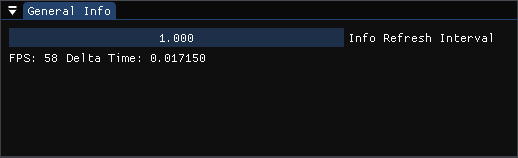
\includegraphics[width=0.9\textwidth]{general_info.png}
    \caption{Prozor za općenite informacije\\}
    \label{fig:general-info}
\end{figure}

\chapter{Implementacija}

Alat je razvijen u programskom jeziku C++ uz korištenje biblioteke OpenGL za komuniciranje sa grafičkom karticom. No, osim OpenGL-a za razvoj alata je korišten i niz drugih biblioteka, čiji su detaljniji opisi i razlozi za korištenje navedeni u poglavlju \ref{libraries-section}. Pošto su se tijekom razvoja alata konstantno pojavljivali novi zahtjevi i funkcionalnosti koje se treba implementirati, potrebno je bilo uspostaviti arhitekturu rješenja koje će se rješenje pridržavati kako ne bi postalo kruto i krhko, a ta arhitektura je opisana u poglavlju \ref{codebase-architecture-section}. Konačno, kako je način slanja podataka sa procesora na grafičku karticu iznimno važna komponenta izvedbe svake grafičke aplikacije, poglavlje \ref{graphics-card-data-section} opisuje kako je organiziran tok podataka sa procesora na grafičku karticu.

\section{Korištene biblioteke} \label{libraries-section}

\subsection{OpenGL}

OpenGL\citep{opengl} je višeplatformska i višejezična biblioteka koja služi za prikazivanje 2D i 3D vektorske grafike. Biblioteka podržava dva distinktna načina rada: \textit{compatibility} i \textit{core}. U \textit{compatibility} načinu rada klijent definira poziciju i boju točaka primitiva koje želi iscrtati pozivajući funkcije API-a, nakon čega se navedene točke propuštaju kroz fiksni grafički protočni sustav na kraju kojega se iscrtava slika. \textit{Core} način rada, često zvani moderni OpenGL, dopušta klijentu mijenjanje određenih dijelova grafičkog protočnog sustava pomoću sjenčara \engl{shader}. Sjenčari su programi napisani u GLSL-u \engl{OpenGL Shading Language} koji se izvode na grafičkoj kartici, te manipuliraju podacima poslanim od strane klijenta preko OpenGL API-a u obliku tzv. \textit{buffer object}-a kako bi se postigli različiti vizualni efekti.\\

Za razvoj alata opisanog u ovom radu je korišten OpenGL 3.3 u \textit{core} načinu rada. Iako je u sklopu implementacije alata ova biblioteka prvenstveno korištena za iscrtavanje 3D modela motora, implementacije biblioteka Dear ImGui (poglavlje \ref{imgui-section}) i ImPlot (poglavlje \ref{implot-section}) korištene u ovom radu također koriste OpenGL za iscrtavanje elemenata korisničkog sučelja i 2D grafova.

\subsection{Dear ImGui} \label{imgui-section}
Dear ImGui\citep{imgui} je C++ biblioteka koja služi za iscrtavanje grafičkog korisničkog sučelja ili GUI-a \engl{Graphical User Interface}.\\

GUI biblioteke se obično mogu razvrstati na zadržane \engl{retained} i izravne \engl{immediate} s obzirom na korištene obrasce ažuriranja prikaza. Zadržane biblioteke interno čuvaju podatke o primitivima korisničkog sučelja koje treba iscrtati, a klijent pozivima metoda biblioteke ne može izravno utjecati na iscrtavanje tih primitiva, već jedino može mijenjati apstraktni model korisničkog sučelja. Na ovakav način zadržane biblioteke mogu dodatno optimizirati kako i kada će se izvršiti iscrtavanje elemenata. S druge strane, izravne GUI biblioteke omogućuju klijentu izravno pozivanje metoda za iscrtavanje elemenata korisničkog sučelja. Zbog toga klijent treba pozivati funkcije za iscrtavanje primitiva u svakoj iteraciji petlje ažuriranja aplikacije.\\

Dear ImGui spada u kategoriju izravnih GUI biblioteka. Ova biblioteka omogućuje jednostavno i brzo iteriranje GUI aplikacija, te unatoč tome što joj nedostaju određene funkcionalnosti koje se mogu naći u drugim GUI bibliotekama, i dalje je iznimno popularna u području razvoja GUI aplikacija zbog jednostavnosti korištenja i nadogradnje.

\subsection{ImPlot} \label{implot-section}

Iako Dear ImGui službeno podržava crtanje grafova, funkcionalnosti grafova implementiranih u sklopu ove biblioteke su iznimno ograničene. Iz tog razloga, za implementaciju grafova u ovom radu je korištena biblioteka ImPlot\citep{implot}. Ova biblioteka je proširenje Dear ImGui-a koje omogućava prikaz raznovrsnih interaktivnih grafova jednostavnim izravnim pozivima metoda za iscrtavanje. 

\subsection{Ostale biblioteke}
Osim već spomenutih biblioteka, za razvoj ovog alata je korištena još nekolicina drugih biblioteka koje su navedene u ovom poglavlju.\\

GLFW\citep{glfw} je višeplatformska biblioteka za razvoj OpenGL aplikacija, a u sklopu ove aplikacije biblioteka je korištena za stvaranje prozora, konteksta, javljanje događaja i primanje ulaza od korisnika.\\

GLM\citep{glm} je matematička biblioteka za grafičke aplikacije pisane u OpenGL-u. GLM nudi brojne klase i funkcije koje su dizajnirane i implementirane sa istim konvencijama imenovanja i funkcionalnostima kao odgovarajući tipovi podataka i funkcije u GLSL-u. GLM je u ovom alatu korišten za operacije nad vektorima, te računanje matrica transformacije i projekcije.\\

NFD\citep{nfd} \engl{Native File Dialog} je višeplatformska C biblioteka koja pruža mogućnost otvaranja izvornog dijaloga za datoteke, a u sklopu alata je korištena prilikom učitavanja različitih datoteka sa podacima o motoru.

\section{Arhitektura rješenja} \label{codebase-architecture-section}

Organizacija koda alata je generalno inspirirana obrascom Model-Pogled-Upravljač ili MVC \engl{Model-View-Controller} kako bi se omogućilo lakše održavanje programa. Na slici \ref{fig:high-level-overview} se može vidjeti pojednostavljeni prikaz MVC organizacije alata sa većinom ključnih klasa alata.

\begin{figure} [H]
	\centering
    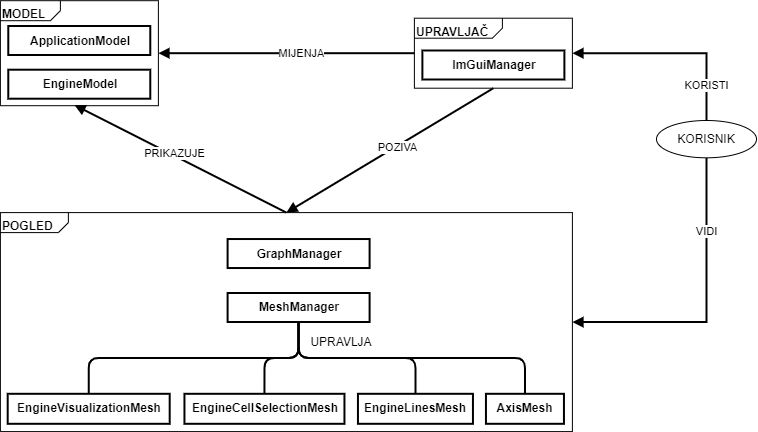
\includegraphics[width=\textwidth]{high_level_overview.png}
    \caption{Pregled MVC organizacije alata}
    \label{fig:high-level-overview}
\end{figure}
\ 
\\

Važno je spomenuti kako na slici \ref{fig:high-level-overview} nedostaje glavna klasa alata, a to je klasa \textit{App}, pošto ne sudjeluje direktno u MVC arhitekturi. Glavna odgovornost ove klase je povezivanje prikazanih komponenti, obrađivanje GLFW događaja i pozivanje metoda za ažuriranje spomenutih komponenti tijekom iteracija petlje ažuriranja. Spomenuta klasa stvara instance komponenti MVC arhitekture, te ih međusobno povezuje slanjem preko argumenata konstruktora ili povezivanjem preko sustava događaja i signala (detaljno opisanih u dodatku \ref{appendix:event-signal-system}). U poglavljima koje slijede su opisane uloge, odgovornosti i dijelovi svake komponente MVC organizacije ovog alata.

\subsection{Model}
Osnovna odgovornost svakog Modela u sklopu MVC arhitekture je čuvanja podataka aplikacije i pravila za njihovu manipulaciju. Radi lakšeg razumijevanja koda i raspodjele odgovornosti, Model ovog alata je podijeljen u dvije klase: \textit{EngineModel} i \textit{ApplicationModel}. Objekt klase \textit{EngineModel} čuva postavke i podatake vezane za motor i prikaz motora, poput odabranih frekvencija, odabranih ćelija, "trenutne" lebdeće ćelije, pozicija točaka motora, ćelija motora itd., te definira metode za mijenjanje navedenih podataka. S druge strane, odgovornost klase \textit{ApplicationModel} je čuvanje postavki aplikacije koje nisu izravno vezane za podatke o motoru ili prikaz tih podataka, te definiranje metoda za vanjsko mijenjanje tih postavki. Spomenute postavke i podaci uključuju razne postavke grafova, postavke bojanja motora, pozadinsku boju alata te poziciju i rotaciju kamere.\\

Navedene klase nemaju izravne reference na nijedan drugi dio MVC arhitekture, stoga svaki put kada se dogodi promjena u Modelu, oni je javljaju "pretplatnicima" na tu promjenu pomoću događaja i/ili signala, čime se smanjuje krutost programskog rješenja. Što se mijenjanja postavki tiče, objekti spomenutih klasa interno sadrže objekte klase \textit{VariableMap} (detaljno opisana u dodatku \ref{appendix:variablemap-class}) čija je odgovornost čuvanje varijabli postavki, te pozivanje zadane metode kada se dogodi promjena u nekoj varijabli. Na taj način su omogućeni povratni pozivi, koje Dear ImGui za većinu elemenata korisničkog sučelja zapravo ne podržava. Kako bi se promjene u Modelu ispitale prilikom svake iteracije petlje ažuriranja alata, već spomenuta klasa \textit{App} poziva odgovarajuće metode objekata klasa \textit{EngineModel} i \textit{ApplicationModel} koje interno zovu metode vlastitih \textit{VariableMap} objekata.

\subsection{Pogled}

Pogled je, kao komponenta MVC-a, uglavnom odgovoran za prikaz podataka iz komponente Model na koristan i praktičan način. Na slici \ref{fig:high-level-overview} se može vidjeti kako je komponenta Pogled, baš kao i Model, podijeljena na dvije klase: \textit{MeshManager} i \textit{GraphManager}.\\

Ključna odgovornost klase \textit{MeshManager} je iscrtavanje poligona i linija uz pomoć OpenGL-a na temelju podataka iz komponente Model. Kako se može vidjeti na skici organizacije arhitekture koda, klasa \textit{MeshManager} to čini uz četiri pomoćne klase: \textit{EngineVisualizationMesh}, \textit{EngineCellSelectionMesh}, \textit{EngineLinesMesh} i \textit{AxisMesh}. Sve navedene pomoćne klase nasljeđuju apstraktnu klasu \textit{AbstractMesh}, s time da sve klase osim klase \textit{AxisMesh} klasu ne nasljeđuju izravno, već preko posredničke apstraktne klase \textit{AbstractEngineMesh}.
Implementirana je i klasa \textit{Shader} kako bi se apstrahirale operacije vezane za sjenčare, a svaka od spomenutih komponenata \textit{MeshManager}-a sadrži vlastitu instancu klase \textit{Shader}, te definira vlastite \textit{buffer object}-e koje šalje na grafičku karticu (više u poglavlju \ref{graphics-card-data-section}).  Rezultati iscrtavanja se ne spremaju u glavni grafički međuspremnik \engl{framebuffer}, već u dva sporedna međuspremnika. U prvi međuspremnik rezultate iscrtavanja upisuju objekti klase \textit{EngineVisualizationMesh}, \textit{EngineLinesMesh} i \textit{AxisMesh}, a to je međuspremnik koji korisnik vidi jer se u prozoru prikaza motora zapravo iscrtava tekstura u koju se spremaju RGB vrijednosti navedenog međuspremnika. 

\subsection{Upravljač}

\section{Organizacija podataka na grafičkoj kartici} \label{graphics-card-data-section}

\chapter{Demonstracija rada alata}
5-7 stranica

\chapter{Zaključak}
1 stranica

\bibliography{literatura}
\bibliographystyle{fer}

\appendix
\chapter{Različiti načini crtanja grafova} \label{appendix:graph-display-examples}

\begin{figure}[H]
	\centering
	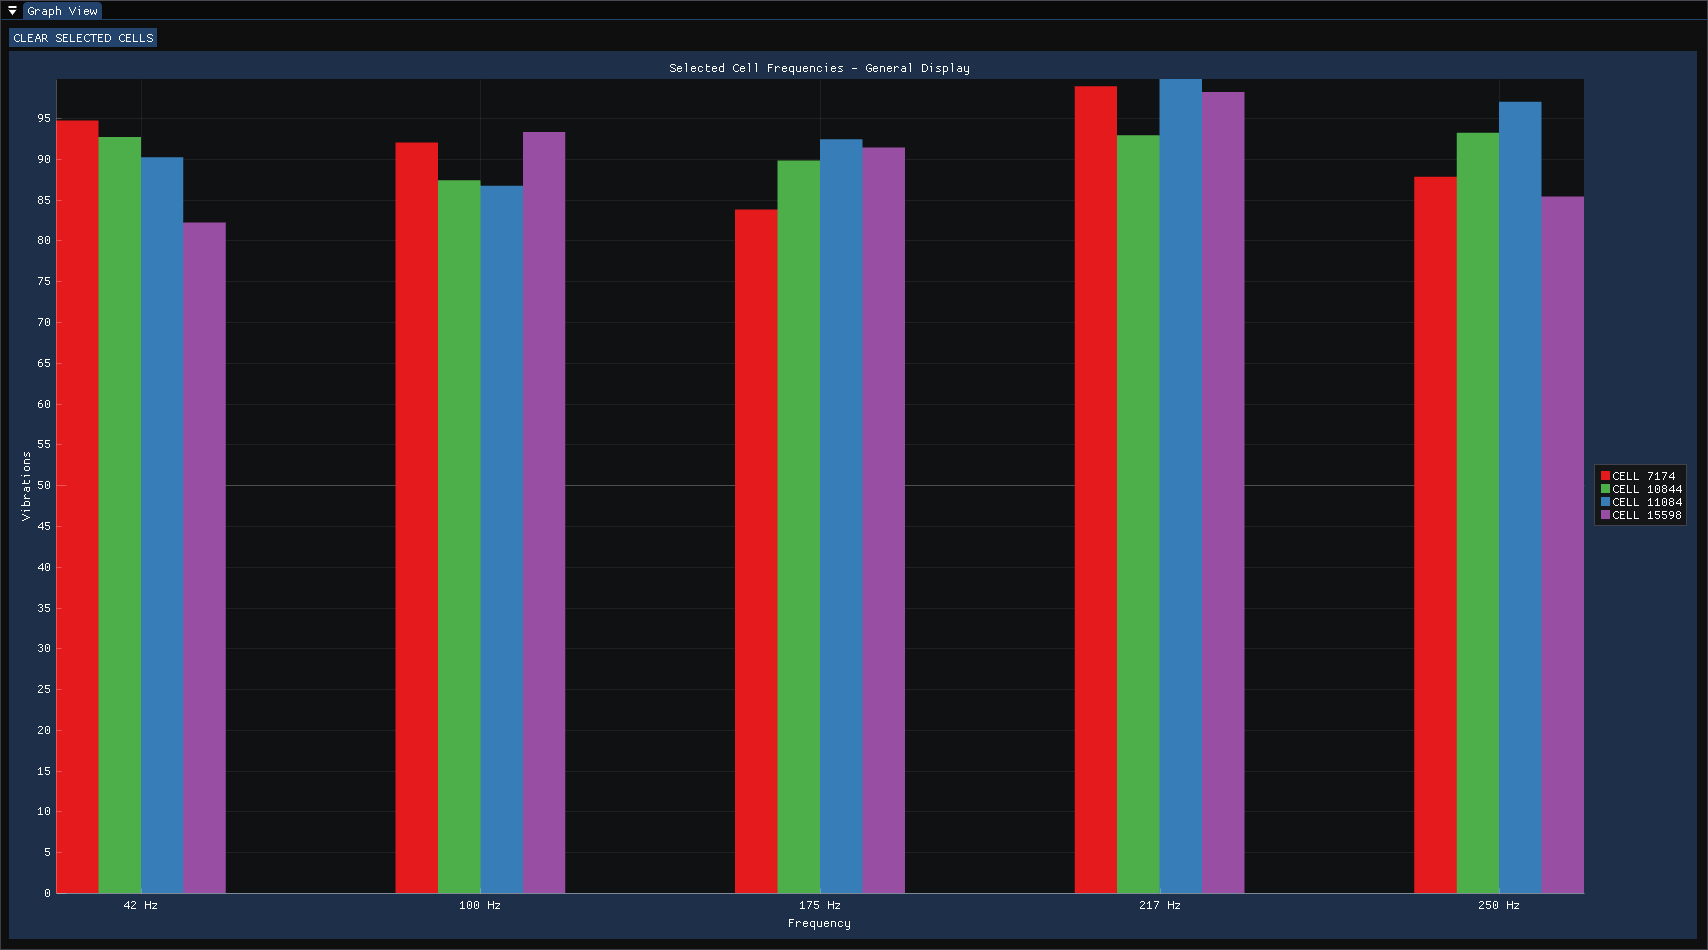
\includegraphics[width=\textwidth]{default_graph_display_bars.png}
	\caption{Normalni način usporedbe grafova u obliku stupaca}
    \label{appendix:default_graph_display_bars}
\end{figure}

\begin{figure}[H]
	\centering
	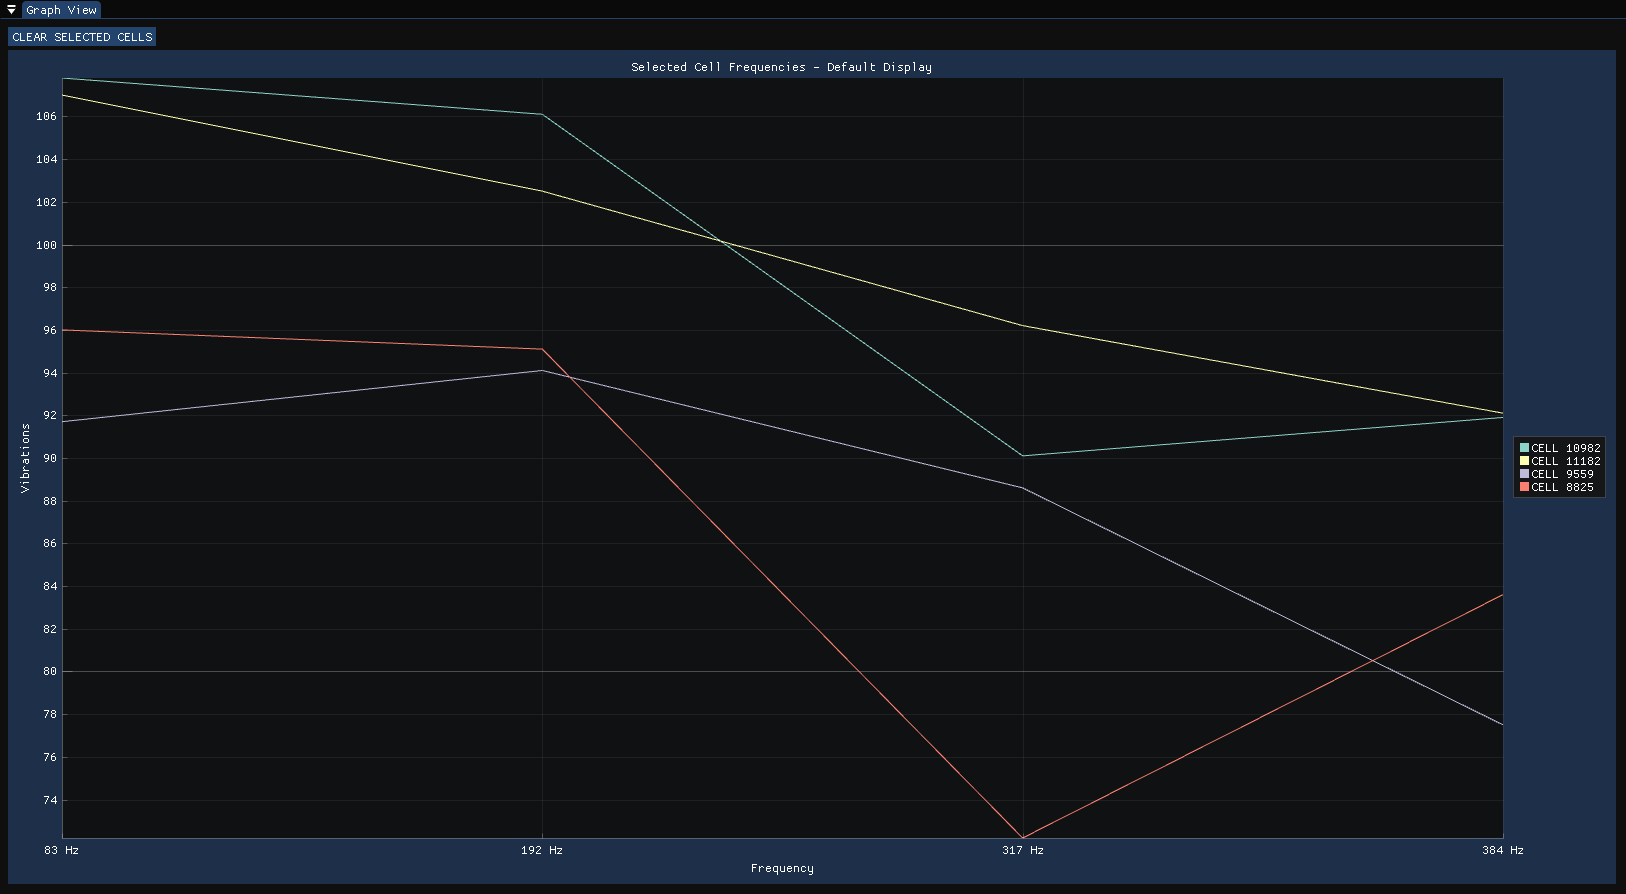
\includegraphics[width=\textwidth]{default_graph_display_lines.png}
	\caption{Normalni način usporedbe grafova u obliku linija}
    \label{appendix:default_graph_display_lines}
\end{figure}

\begin{figure}[H]
	\centering
	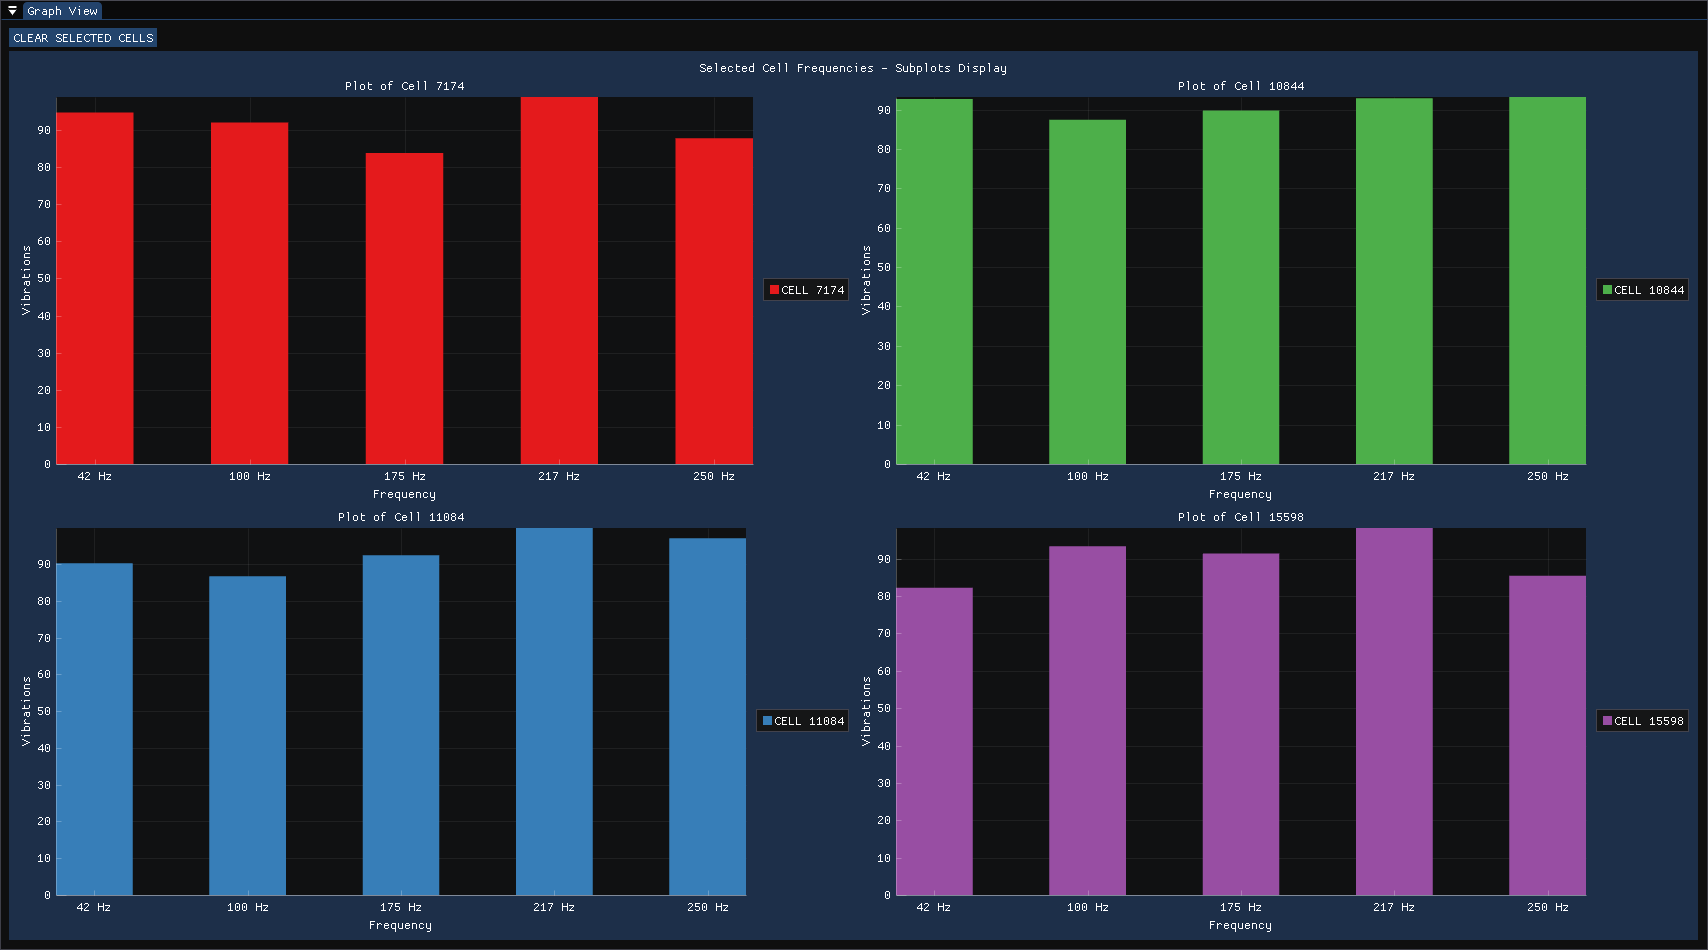
\includegraphics[width=\textwidth]{subplots_graph_display_bars.png}
	\caption{Način usporedbe grafova sa višestrukim prikazima u obliku stupaca}
    \label{appendix:subplots_graph_display_bars}
\end{figure}

\begin{figure}[H]
	\centering
	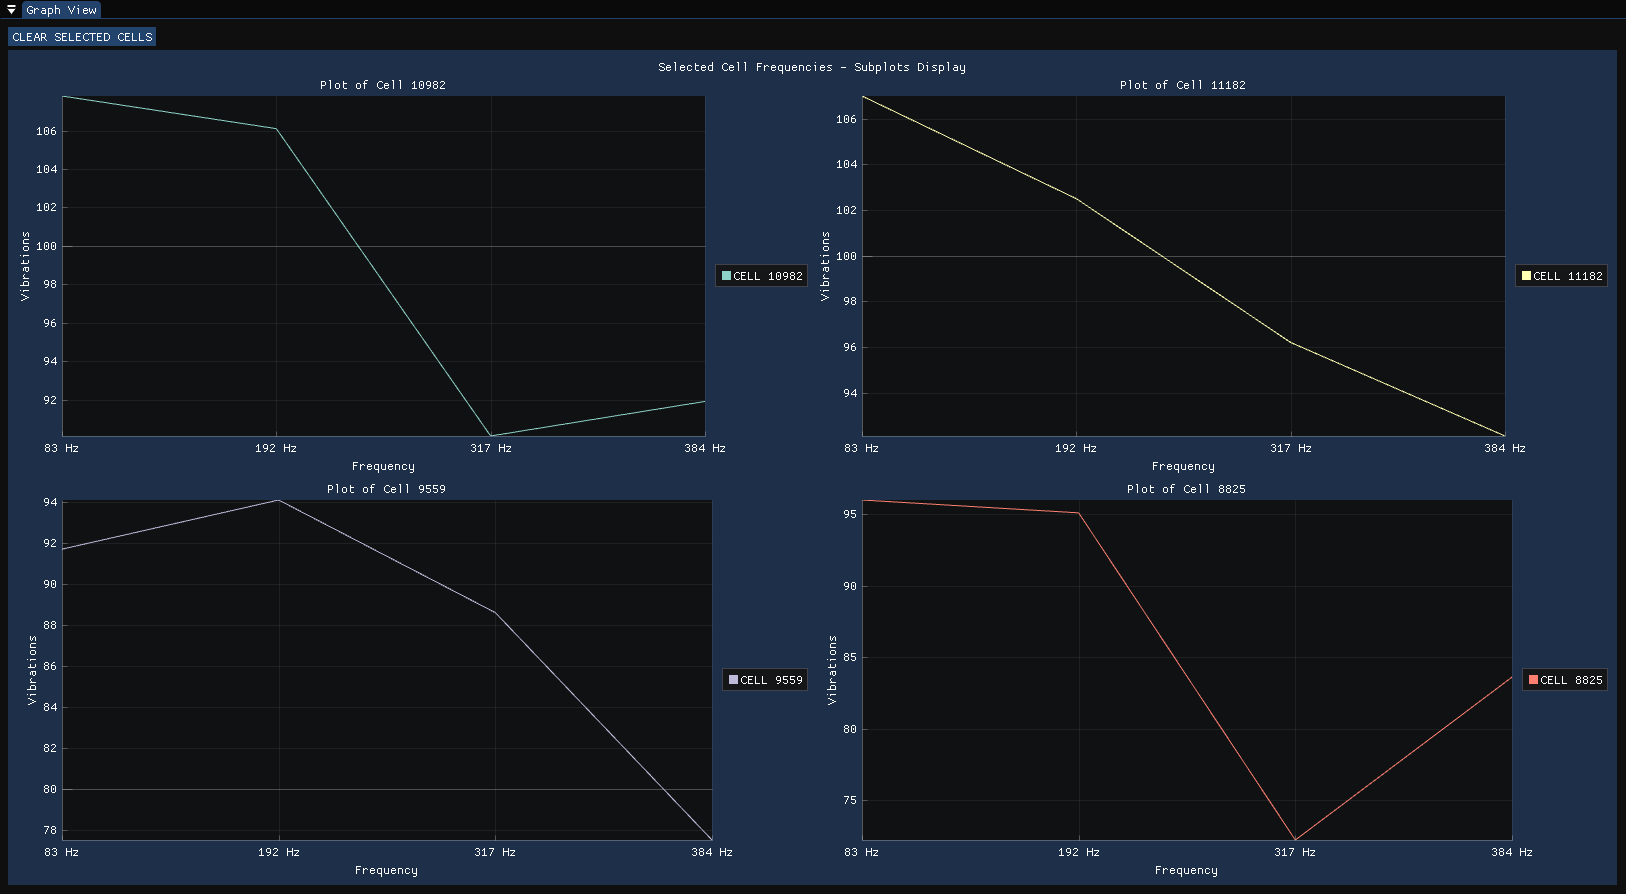
\includegraphics[width=\textwidth]{subplots_graph_display_lines.png}
	\caption{Način usporedbe grafova sa višestrukim prikazima u obliku linija}
    \label{appendix:subplots_graph_display_lines}
\end{figure}

\begin{figure}[H]
	\centering
	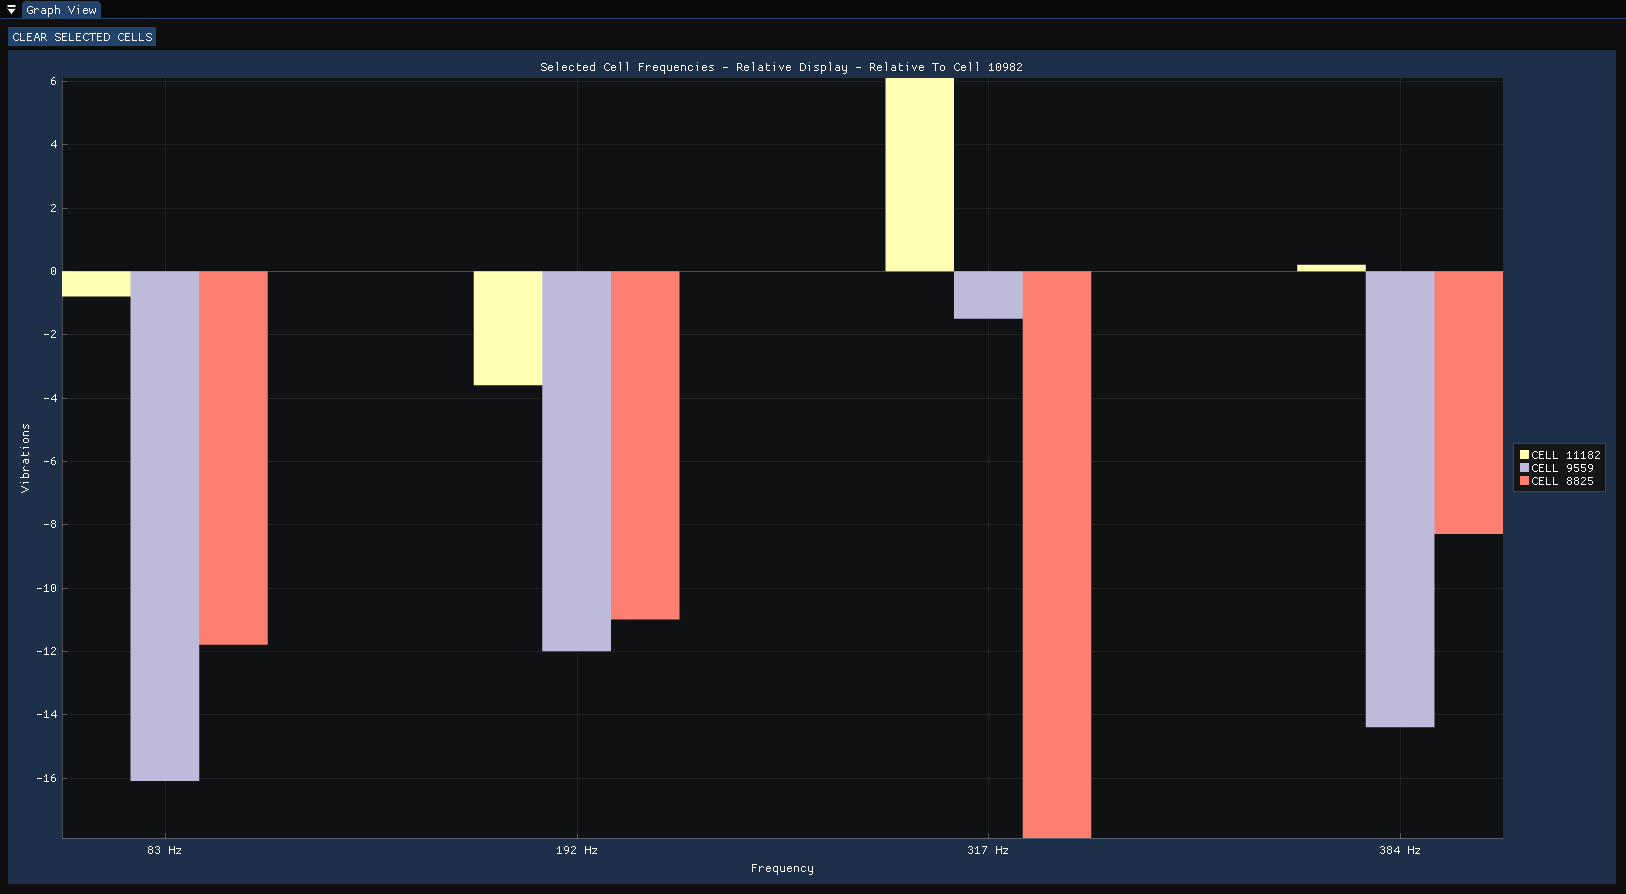
\includegraphics[width=\textwidth]{relative_graph_display_bars_cell_10982.png}
	\caption{Relativni način usporedbe grafova u obliku stupaca u kojem su podaci svih ćelija prikazani u odnosu na ćeliju 10982}
    \label{appendix:relative_graph_display_bars}
\end{figure}

\begin{figure}[H]
	\centering
	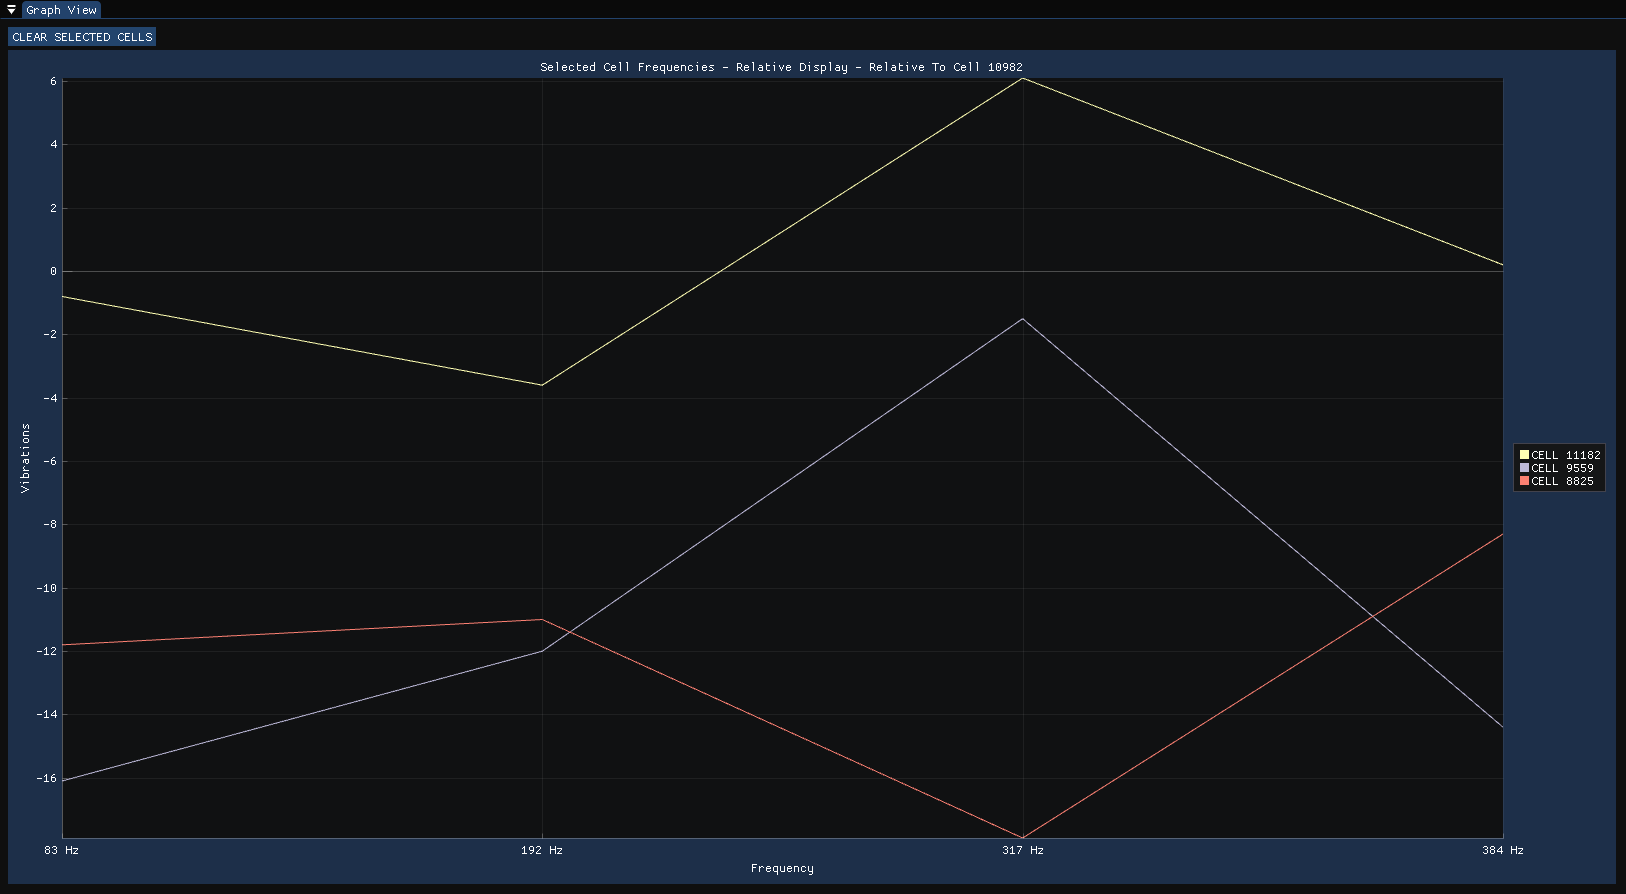
\includegraphics[width=\textwidth]{relative_graph_display_lines_cell_10982.png}
	\caption{Relativni način usporedbe grafova u obliku linija u kojem su podaci svih ćelija prikazani u odnosu na ćeliju 10982}
    \label{appendix:relative_graph_display_lines}
\end{figure}

\chapter{Sustav događaja i signala} \label{appendix:event-signal-system}

\chapter{Klasa \textit{VariableMap}} \label{appendix:variablemap-class}

\begin{sazetak}
Sažetak na hrvatskom jeziku.

\kljucnerijeci{Ključne riječi, odvojene zarezima.}
\end{sazetak}

% TODO: Navedite naslov na engleskom jeziku.
\engtitle{3D Interactive Visualization of Vibration Simulation}
\begin{abstract}
Abstract.

\keywords{Keywords.}
\end{abstract}

\end{document}
